\documentclass[a4paper]{article}

\usepackage[utf8]{inputenc}
\usepackage[portuges]{babel}
\usepackage{a4wide}
\usepackage{graphicx}
\usepackage{underscore}
\usepackage{subcaption}
\usepackage{float}

\title{Projeto de Sistemas Operativos - Processamento de Notebooks }
\author{Diogo Miguel Alves Rocha (A79751)\and Ricardo Milhazes Veloso (A81919) \and Ricardo Jorge Silva Ferreira (82568)}


\date{\today}
\begin{document}

\maketitle

Neste relatório faremos a análise ao nosso projeto de Sistemas Operativos, no qual consiste desenvolver um programa em C, de Processamento de Notebooks. Este documento tem como objetivo apresentar detalhadamente o tipo de abordagem ao problema proposto pela equipa docente.

\tableofcontents

\pagebreak

\section{Introdução}
\label{sec:intro}
Este projeto foi desenvolvido com o objetivo de desenvolver um programa responsável pelo processamento de Notebooks.

\section{Descrição do Problema}
\label{sec:descricao do problema}
Nesta secção mostramos uma parte do enunciado do projeto, onde é demonstrado o resultado final pretendido.

\begin{figure}[H]
				\centering
				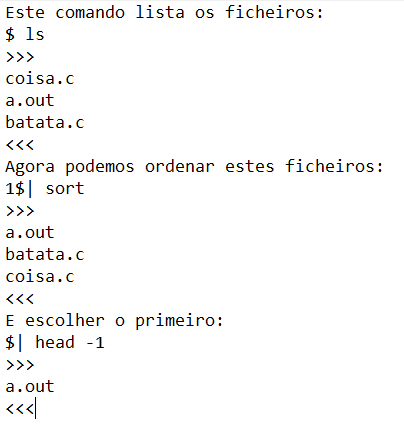
\includegraphics[width = 250pt,height = 150pt]{so.png}
				\caption{Problema}
			\end{figure}


\section{Concepção da Solução}
\label{sec:solucao}

\subsection{AgrupaComando}
A função AgrupaComando transforma uma String (linha) de comandos em um arraylist de comandos.
A função recebe uma linha de comandos.
A função strdup recebe uma linha e retorna uma copia desta
A função strtok recebe uma string (cópia da linha) e um array vazio e atraves do while,retorna um array preenchido em que cada elemento desse array é um comando da linha de comandos lida.

\subsection{fazEcho}
Função que imprime uma string com todos os comandos lidos.


\subsection{executar}
A função executar executa um comando e escreve no ficheiro.
A funçao inicia a função agrupaComando para repartir os comandos pedidos escreve no ficheiro através de pipes o resultado obtido.



\subsection{lerFicheiro}
Função que escreve o ficheiro todo.

\subsection{main}
A funçao inicializa 4 ficheiros distintos e retorna erros se a criaçao de algum nao for bem sucedida
A funçao inicializa uma nova funçao chamada lerFicheiro em que sao passados como argumentos dois ficheiros.

\section{Conclusão}
\label{sec:conclusao}
Este projeto serviu para aprofundarmos os nossos conhecimentos na linguagem C, um trabalho que permite aplicar no mundo real os temas abordados em SO.
Foi um trabalho em que o grupo funcionou bastante bem, apenas a apontar o facto de não termos conseguido cumprir os objetivos propostos nas funcionalidades avançadas.

\end{document}